%%%Theory
\label{ch:theory_overview}

The Standard Model of particle physics is our best description of elementary particles and how they interact. The SM has been tested and proven right by many experiments worldwide at various energy levels. Even though the SM has been very successful, it doesn't answer every question about the universe, leaving space for new theories beyond the SM that try to fill these gaps and explain the mysteries. This chapter gives a simple overview of the SM, discusses the importance of the Higgs field, and explains why studying VBS and aQGCs is essential.

\section{Standard Model}
The Standard Model of particle physics offers a comprehensive framework that describe the fundamental particles and the interactions governing them, excluding gravity~\cite{PeskinSchroeder1995}. 
Table~\ref{table:fundamental_forces} shows the relative strengths of these four fundamental forces, highlighting the marked disparity between gravity and the other forces within the realm of subatomic particles.


\begin{table}[h]
\centering
\begin{tabular}{|l|l|}
\hline
\textbf{Force}         & \textbf{Relative Strength} \\ \hline
Strong Nuclear Force   & 1                          \\ \hline
Electromagnetic Force  & \textasciitilde{}1/137     \\ \hline
Weak Nuclear Force     & \textasciitilde{}10\(^{-6}\) \\ \hline
Gravitational Force    & \textasciitilde{}10\(^{-38}\) \\ \hline
\end{tabular}
\caption{Relative Strengths of the Fundamental Forces}
\label{table:fundamental_forces}
\end{table}


The particles of the Standard Model are classified into four distinct categories. Leptons and quarks constitute all known matter, each possessing half-integer spin and adhering to Fermi-Dirac statistics. This principle prohibits any two identical fermions from occupying identical quantum states simultaneously. The model includes six leptons and six quarks, each accompanied by a corresponding antiparticle counterpart. A fundamental distinction between these particle types is that quarks are subject to the strong nuclear force, whereas leptons are not. Furthermore, quarks are perpetually bound within composite particles known as hadrons—protons and neutrons being the most recognized examples.

The remaining particles within the Standard Model facilitate the interactions among leptons and quarks and are characterized by integer spin, thereby following Bose-Einstein statistics. This group encompasses the gauge bosons, which are spin-1 particles responsible for mediating the three fundamental forces, and the Higgs boson~\cite{Higgs:1964ia}, a unique scalar particle with a spin-0, crucial for imparting mass to other particles. 
Figure~\ref{fig:stdm_higgs} and Table~\ref{table:SMparticles} show all Standard Model particles, alongside their properties.

%figures/theory/STDM_higgs.png

\begin{figure}[ht]
    \centering
%%    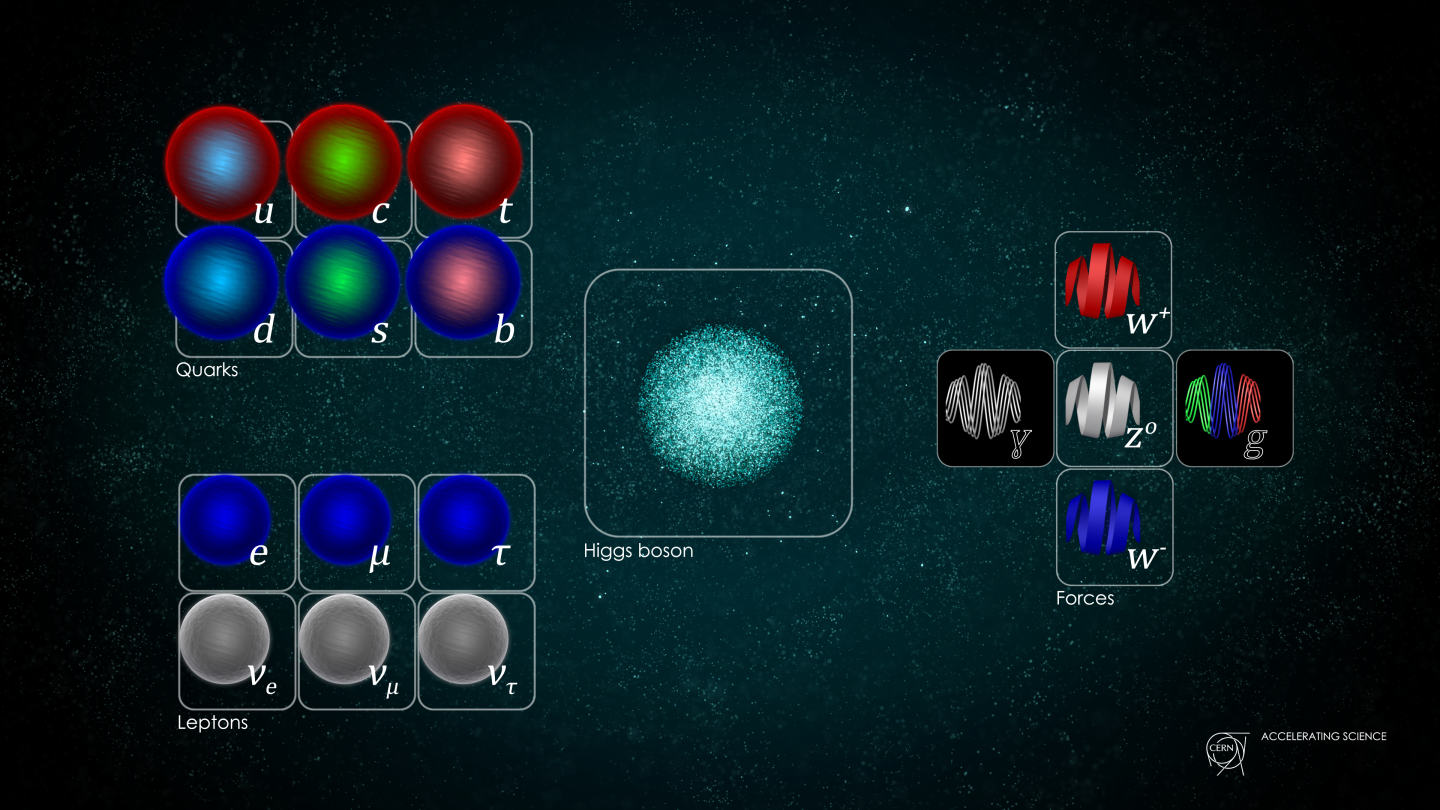
\includegraphics[width=0.95\textwidth]{figures/theory/STDM_higgs.png}
    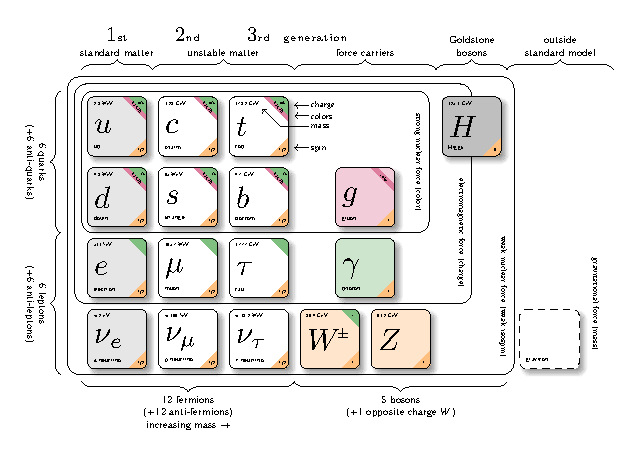
\includegraphics[width=0.95\textwidth]{figures/theory/model-physics.pdf}
    \caption{Illustration of Standard Model particles~\cite{Burgard2019}.}
    \label{fig:stdm_higgs}
\end{figure}

\begin{table}[ht]
\centering
\begin{tabular}{|l|l|l|l|l|}
\hline
\textbf{Particle Type} & \textbf{Particle} & \textbf{Spin} & \textbf{Charge (e)} & \textbf{Mass}            \\ \hline
\multirow{6}{*}{Lepton}& Electron (e\(^-\))        & 1/2           & -1               & 0.511 MeV/c\(^2\)        \\ \cline{2-5}
                       & Muon (\(\mu^-\))          & 1/2           & -1               & 105.7 MeV/c\(^2\)        \\ \cline{2-5}
                       & Tau (\(\tau^-\))          & 1/2           & -1               & 1.777 GeV/c\(^2\)        \\ \cline{2-5}
                       & Electron Neutrino (\(\nu_e\))    & 1/2           & 0                & $< 2 \, \text{eV}/c^2$           \\ \cline{2-5}
                       & Muon Neutrino (\(\nu_{\mu}\))    & 1/2           & 0                & $< 0.19 \, \text{MeV}/c^2$       \\ \cline{2-5}
                       & Tau Neutrino (\(\nu_{\tau}\))    & 1/2           & 0                & $< 18.2 \, \text{MeV}/c^2$       \\ \hline
\multirow{6}{*}{Quark} & Up (u)                & 1/2           & +2/3              & 2.3 MeV/c\(^2\)          \\ \cline{2-5}
                       & Down (d)              & 1/2           & -1/3              & 4.8 MeV/c\(^2\)          \\ \cline{2-5}
                       & Charm (c)             & 1/2           & +2/3              & 1.275 GeV/c\(^2\)        \\ \cline{2-5}
                       & Strange (s)           & 1/2           & -1/3              & 95 MeV/c\(^2\)           \\ \cline{2-5}
                       & Top (t)               & 1/2           & +2/3              & 173.1 GeV/c\(^2\)        \\ \cline{2-5}
                       & Bottom (b)            & 1/2           & -1/3              & 4.18 GeV/c\(^2\)         \\ \hline
\multirow{4}{*}{Gauge Boson} & Photon (\(\gamma\))         & 1             & 0                & 0                        \\ \cline{2-5}
                       & W Boson (W\(^{\pm}\))       & 1             & \(\pm 1\)        & 80.379 GeV/c\(^2\)       \\ \cline{2-5}
                       & Z Boson (Z\(^0\))          & 1             & 0                & 91.1876 GeV/c\(^2\)       \\ \cline{2-5}
                       & Gluon (g)             & 1             & 0                & 0                         \\ \hline
Scalar Boson           & Higgs (H)             & 0             & 0                & 125.10 GeV/c\(^2\)       \\ \hline
\end{tabular}
\caption{Standard Model Particles and Their Known Properties.}
\label{table:SMparticles}
\end{table}

\label{subsec:qcd}
The SM is a quantum field theory anchored in the symmetry group $\mathrm{SU}(3)_C \otimes \mathrm{SU}(2)_L \otimes \mathrm{U}(1)_Y$, where each component of the symmetry group governs a different aspect of particle interactions. In this context, the $\mathrm{SU}(3)_C$ symmetry relates to the strong interaction, with the subscript $C$ denoting color charge—a conserved property. Color charge exists in three forms—red, blue, and green—alongside their anticolors (anti-red, anti-blue, and anti-green).

One of the foundational principles of quantum chromodynamics (QCD)~\cite{CampbellHustonKrauss2017}, the theory of the strong interaction, is that color charge is never observed in isolation. This phenomenon, known as color confinement, dictates that quarks are always found in composite particles called hadrons, which exhibit a neutral color charge. 
Hadrons are categorized into mesons and baryons. Mesons consist of a quark and an antiquark pair, combining a color with its anticolor. Baryons, such as the proton and neutron, are formed from three quarks, each of a distinct color (or anticolor), which collectively neutralize their color charge. This configuration explains why hadrons are observable in nature, contrary to isolated quarks.
As quarks attempt to separate, they undergo a process known as \emph{hadronization}. During hadronization, new quark-antiquark pairs spontaneously emerge from the vacuum. These new particles arrange themselves to neutralize the color charge of the initially separating quarks. As a result, instead of isolated quarks, we observe the formation of new hadrons, ensuring that the color charge remains confined.
Hadronization and its resulting particle decays produce a shower(cascade) of hadrons and leptons known as a ``jet.'' These jets, which will be discussed on in Section~\ref{subsec:jet_selection}, are crucial for probing QCD physics. 

The electroweak interaction, described by the symmetry group $\mathrm{SU}(2)_L \times \mathrm{U}(1)_Y$, unifies the electromagnetic and weak forces~\cite{GLASHOW1961579, PhysRev.127.965, PhysRevLett.19.1264}. The conservation of electric charge ($Q$) is central to this theory, governed by the formula: $Q = \frac{Y}{2} + T_3$. Here, $Y$ denotes the hypercharge, and $T_3$ is the third component of the weak isospin ($T$), akin to the third component of spin in quantum mechanics, differentiating ``up'' and ``down'' states within isospin doublets. This framework introduces a distinction in symmetry for particles based on their chirality: left-handed particles exhibit doublet configurations under $\mathrm{SU}(2)_L$, while right-handed particles form singlets, indicating they do not participate in weak isospin doublets. 

Spin-1 particles, known as gauge bosons or vector bosons, are the force carriers in the SM. The photon mediates the electromagnetic force. The weak force is mediated by three vector bosons, the $W^{\pm}$ and $Z$ bosons. For the strong force, it is mediated by eight different gluons. A key feature of the weak force is lepton universality, meaning all types of leptons couple to the $W^{\pm}$ and $Z$ bosons in the same way, leading to identical branching ratios for each lepton type.

\section{The Higgs Mechanism}

%%%Higgs

In the SM, the requirement of gauge invariance under the group $\mathrm{SU}(2)_L \otimes \mathrm{U}(1)_Y$ implies that weak bosons and fermions should be massless. However, this stands in contradiction to the observed masses of these particles. 
The resolution within the SM framework is the Higgs mechanism \cite{Higgs:1964ia, PhysRevLett.13.508, PhysRevLett.13.321, PhysRevLett.13.585}, which introduces the Higgs field. Through spontaneous symmetry breaking, this scalar field gives mass to the weak bosons and fermions, reconciling the SM with experimental observations.

Spontaneous symmetry breaking refers to a phenomenon where the ground state of a symmetric system does not reflect the system's symmetry after perturbation. The term ``breaking'' does not imply the destruction of the Lagrangian symmetry. Instead, the symmetry is not apparent in the perturbed ground state of the system.
A classical example of spontaneous symmetry breaking is the magnetization of iron. Above its Curie temperature, iron's magnetic moments are oriented randomly, respecting rotational symmetry. Upon cooling below this temperature, the moments align uniformly, creating a magnet with distinct poles. Although the magnet displays a specific orientation, the physical principles governing magnetism retain their inherent symmetry.

The scalar field (Higgs field), $\phi$, represented as a complex doublet, takes on a non-zero vacuum expectation value (VEV) of $v \approx 246$ GeV, leading to three massive gauge bosons ($W^{\pm}$ and $Z$) and the Higgs boson ($H$).

% The complex scalar doublet
\begin{equation}
\phi =
\begin{pmatrix}
\phi^+ \\
\phi^0
\end{pmatrix}
=
\frac{1}{\sqrt{2}}
\begin{pmatrix}
\phi_1 + i\phi_2 \\
\phi_3 + i\phi_4
\end{pmatrix}
\end{equation}



The Lagrangian density of the Higgs field, $\mathcal{L}_\text{Higgs}$, respects local $\mathrm{SU}(2)_L \otimes \mathrm{U}(1)_Y$ symmetry and includes the Higgs potential $V(\phi)$, as shown in Figure~\ref{fig:higgs_potential}. This potential is defined with parameters $\mu^2 < 0$ and $\lambda > 0$ to ensure stable minima. 
% The Lagrangian density
\begin{equation}
\mathcal{L}_\text{Higgs} = (D^\mu\phi)^\dagger (D_\mu\phi) - V(\phi),
\end{equation}
where \(V(\phi)\) is the Higgs potential, given by
\begin{equation}
V(\phi) = \mu^2\phi^\dagger\phi + \lambda (\phi^\dagger\phi)^2.
\end{equation}

\begin{figure}[ht]
\centering
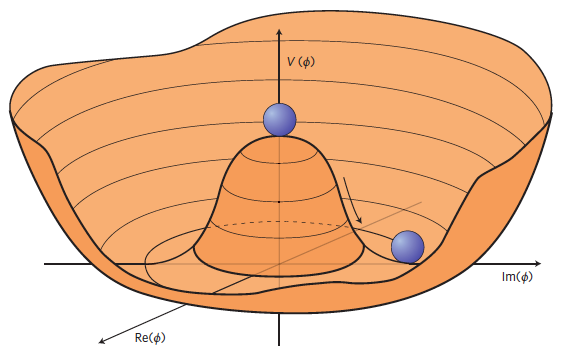
\includegraphics[width=0.75\textwidth]{figures/theory/higgspotential.png}
\caption[Higgs Potential]{The Higgs potential, adapted from Ellis (2013) \cite{ellis2013higgs}.}
\label{fig:higgs_potential}
\end{figure}

Choosing a ground state breaks the $\mathrm{SU}(2)_L \otimes \mathrm{U}(1)_Y$ symmetry to the subgroup $\mathrm{U}(1)_\text{QED}$, reparameterizing the complex scalar doublet's components into observable fields.
After this symmetry breaking, the scalar doublet fields are reparameterized as:
\begin{equation}
\phi(x) = \frac{1}{\sqrt{2}}
\begin{pmatrix}
0 \\
v + h(x)
\end{pmatrix}
\exp\left( \frac{i \tau^i \phi^i(x)}{2} \right),
\end{equation}
where $h(x)$ is the Higgs boson field, and the $\phi^i(x)$ are the Goldstone bosons that become gauge degrees of freedom in the unitary gauge $\phi^i(x) = 0$. This simplifies the kinetic term of the Lagrangian, resulting in mass terms for the $W^\pm$ and $Z$ bosons as:
\begin{equation}
m_W = \frac{1}{2}vg, \quad m_Z = \frac{vg}{2\cos\theta_W}.
\end{equation}
The Higgs boson mass is determined as:
\begin{equation}
m_h = \sqrt{-2\mu^2} = v\sqrt{2\lambda}.
\end{equation}

In the SM, the VEV of the Higgs field, denoted by \( v \), along with the gauge coupling constants \( g_1 \) and \( g_2 \), are free parameters. These are not predicted by the theory but are determined through experimental measurements. The VEV has been established to be about 246 GeV~\cite{Plehn_2005}. This VEV is crucial as it gives mass to the $W^\pm$ and $Z$ bosons through the mechanism previously discussed.

Quarks and charged leptons also gain their mass by interacting with the Higgs field. These interactions are described by Yukawa couplings~\cite{10.1143/PTPS.1.1}.
Each type of fermion has its own Yukawa coupling constant \( c_i \), which determines the strength of its interaction with the Higgs field, and therefore, its mass.


\begin{equation}
\mathcal{L}_\text{Yukawa} = -\frac{1}{\sqrt{2}} (v + h)(c_{1} \bar{d}d + c_{2} \bar{u}u + c_{3} \bar{e}e)
\end{equation}

\begin{equation}
= -\left( 1 + \frac{h}{v} \right)(m_{d} \bar{d}d + m_{u} \bar{u}u + m_{e} \bar{e}e) .
\end{equation}


Neutrinos, however, do not acquire mass through the same mechanism. They remain massless in the SM's framework of electroweak symmetry breaking. The fact that neutrinos have been observed to have mass in experiments is an unsolved issue within the SM, hinting at new physics beyond the current theory.

\section{Vector Boson Scattering}
%%%VBS Theory
%\section{Vector Boson Scattering}
\label{section:Vector_Boson_Scattering}

When the scalar field \( \phi \) is expanded around its ground state value, the kinetic term in $\mathcal{L}_\text{Higgs}$ becomes

\begin{equation}
|D_\mu \phi|^2 = \frac{1}{2} (\partial_\mu \phi_0)^2 + \frac{1}{2} (\partial_\mu \phi_2)^2 
+ g^2 \phi_0^2 A_\mu A^\mu + \sqrt{2} g \phi_0 A_\mu \partial^\mu \phi_2 + \ldots,
\end{equation}
where the mass term for \( A_\mu \) is \( g^2 \phi_0^2 A_\mu A^\mu \). The term \( \sqrt{2} g \phi_0 A_\mu \partial^\mu \phi_2 \) provides an extra degree of freedom for \( A_\mu \). The directly coupling \( A_\mu \) to \( \phi_2 \) allows \( \phi_2 \) to serve as an additional degree of freedom for the gauge boson \( A_\mu \), enabling it to acquire the necessary longitudinal polarization to be a massive particle.

A vector boson is a boson with spin-1. By definition, the gauge bosons mentioned above are vector bosons, which introduces Vector Boson Scattering (VBS) into the discussion. 
The SM VBS process involves a quartic gauge coupling (QGC) vertex, as shown in Figure~\ref{fig:qgc_vertex}, which depicts the self-coupling among four electroweak gauge bosons.
The discovery of a Higgs boson in LHC~\cite{20121, 201230} motivates further study of the mechanism of EWSB by probing the VBS processes.
Given that new physics in the electroweak sector is likely to involve QGCs,
the measurements of VBS at high energy are crucial tests of the SM and will determine whether the Higgs is entirely responsible for EWSB.

\begin{figure}[tbp]
\centering
\subfloat[]{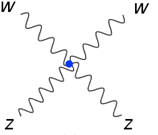
\includegraphics[width=0.27\textwidth]{figures/theory/qgc_1.png}}
\hfill
\subfloat[]{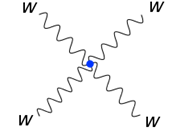
\includegraphics[width=0.3\textwidth]{figures/theory/qgc_2.png}}
\hfill
\subfloat[]{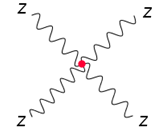
\includegraphics[width=0.27\textwidth]{figures/theory/qgc_3.png}}
\caption{Examples of QGC vertices: (a) and (b) are within the SM; (c) is anomalous, discussed further in Section~\ref{Anomalous_Quartic_Gauge_Couplings}. These and other Feynman diagrams in this thesis are made using the JaxoDraw~\cite{Binosi:2003yf} program.}
\label{fig:qgc_vertex}
\end{figure}

In Figure~\ref{fig:feynmanVBS}, we present examples of VBS diagrams that contribute to the SM signal process in the analysis. 
In the Feynman diagrams presented, a dashed line represents the Higgs boson, a solid line represents quark, and a rippled line represents vector boson.
It's noteworthy that not all VBS diagrams involve quartic gauge couplings. The decays of the bosons are not explicitly shown.

In Figure~\ref{fig:feynmanEWKnonVBS}, we present several non-VBS electroweak diagrams. These include purely-electroweak tree-level diagrams, specifically of order $\mathcal{O}(\alpha_{EW}^6)$, contributing to the final state. Such non-VBS diagrams are expected to be significantly suppressed by the event selection criteria employed in this analysis.

%% feynman diagrams, VBS
%
\begin{figure}[tbp]
\begin{center}
\subfloat[]{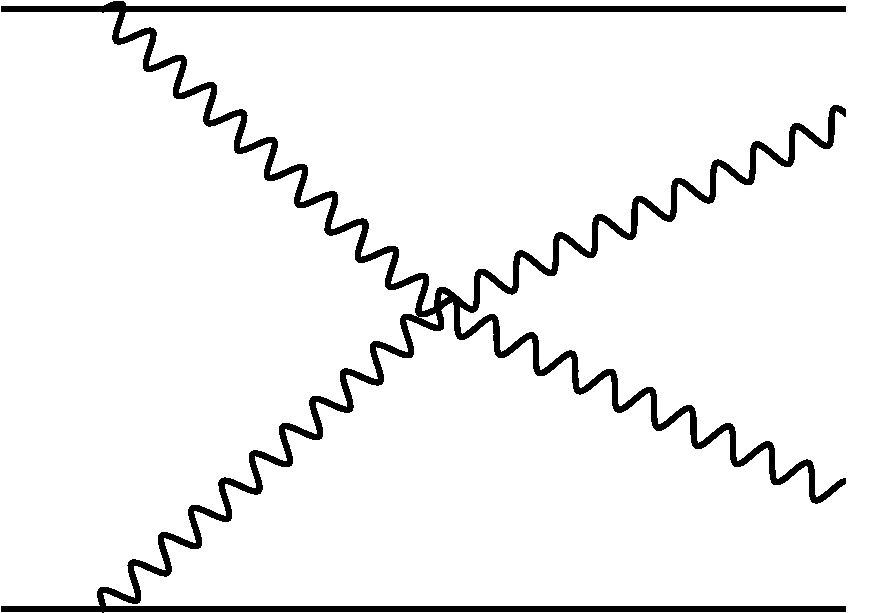
\includegraphics[width=0.3\textwidth]{figures/samples/feynVBS2.pdf}}
\subfloat[]{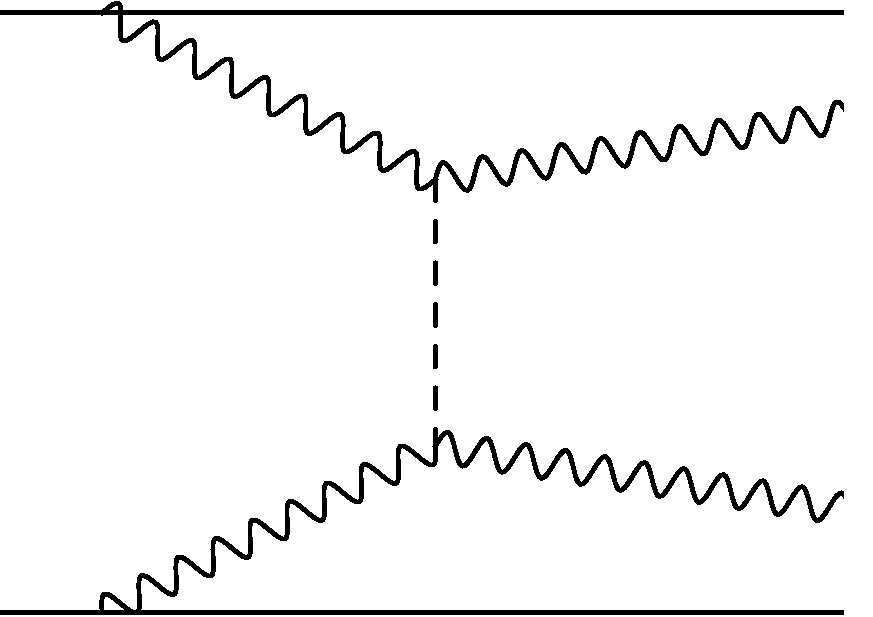
\includegraphics[width=0.3\textwidth]{figures/samples/feynVBS1.pdf}}
\subfloat[]{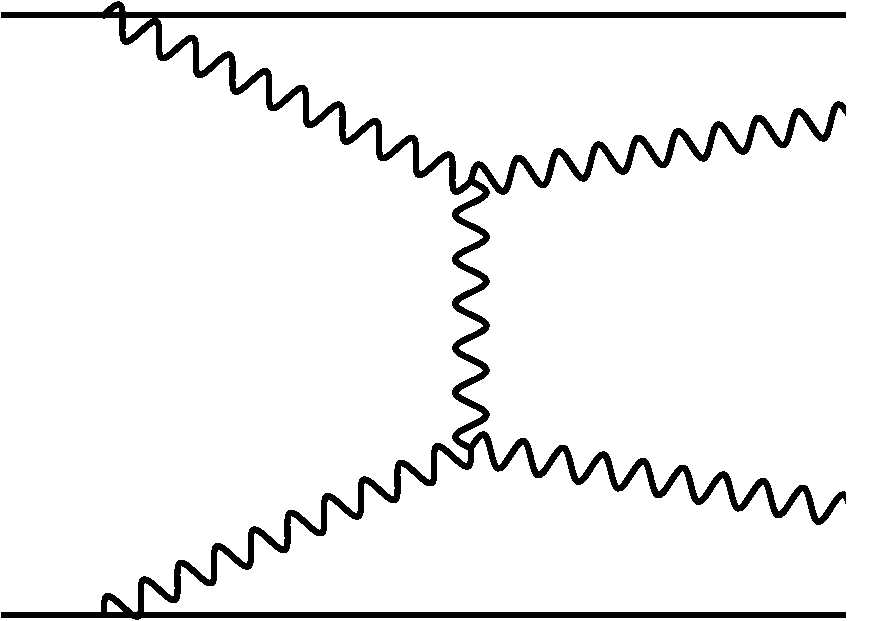
\includegraphics[width=0.3\textwidth]{figures/samples/feynVBS3.pdf}}\\
\subfloat[]{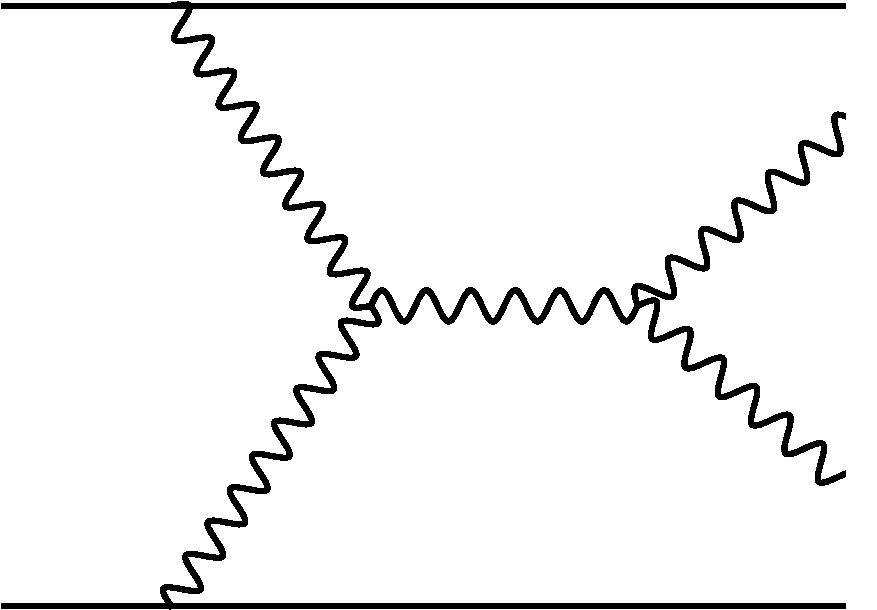
\includegraphics[width=0.3\textwidth]{figures/samples/feynVBS4.pdf}}
\subfloat[]{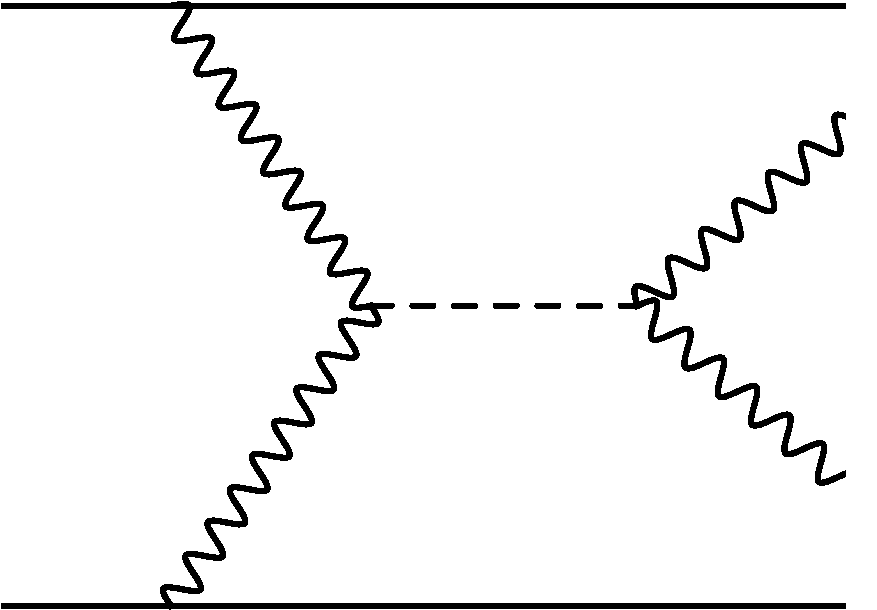
\includegraphics[width=0.3\textwidth]{figures/samples/feynVBS5.pdf}}
\caption{
Examples of VBS diagrams contributing to the signal. Note that not all VBS diagrams contain quartic gauge couplings.
}
\label{fig:feynmanVBS}
\end{center}
\end{figure}


%% feynman diagrams, non-VBS
%
\begin{figure}[tbp]
\begin{center}
\subfloat[]{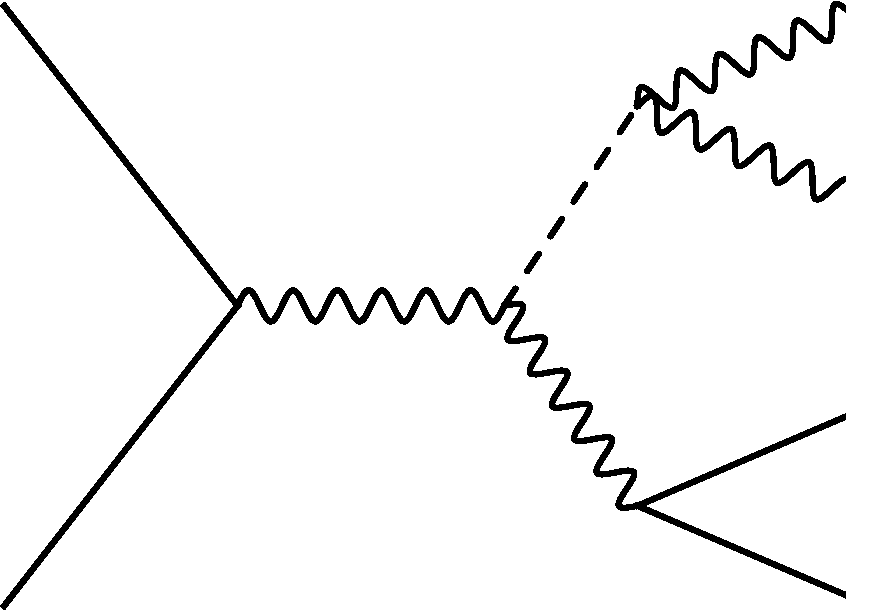
\includegraphics[width=0.3\textwidth]{figures/samples/feynEWKnonVBS3.pdf}}
\subfloat[\label{subfig:feynEWKnonVBSb}]{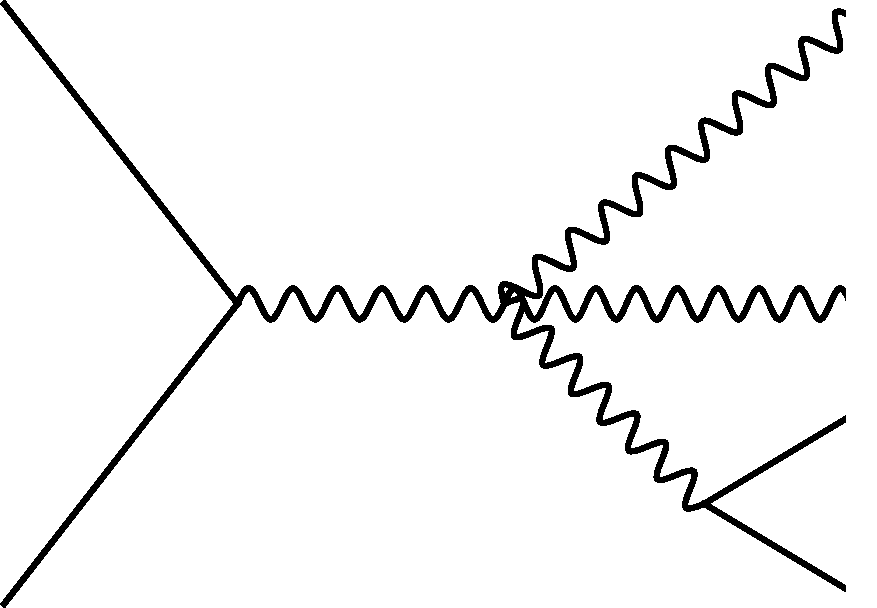
\includegraphics[width=0.3\textwidth]{figures/samples/feynEWKnonVBS4.pdf}}
\subfloat[]{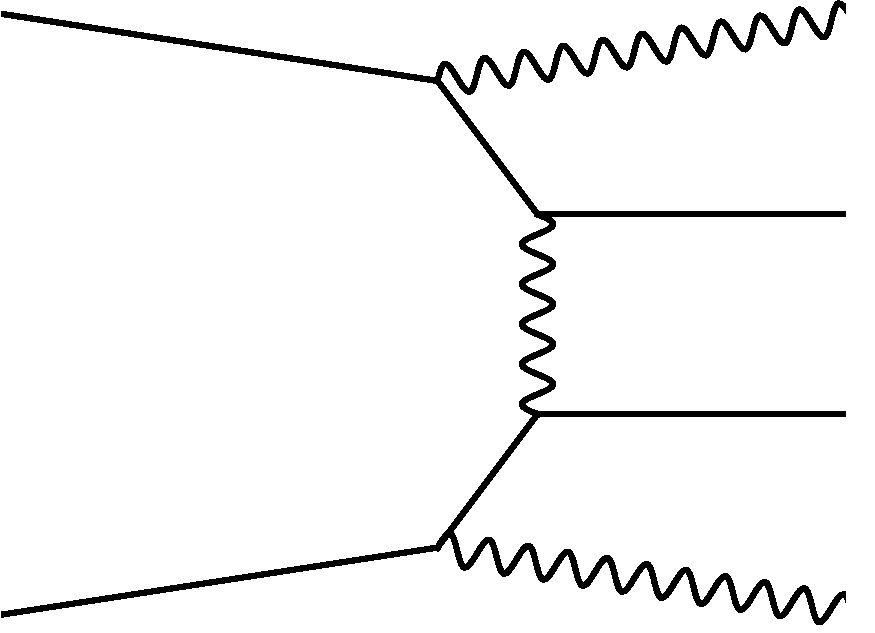
\includegraphics[width=0.3\textwidth]{figures/samples/feynEWKnonVBS5.pdf}}\\
\subfloat[]{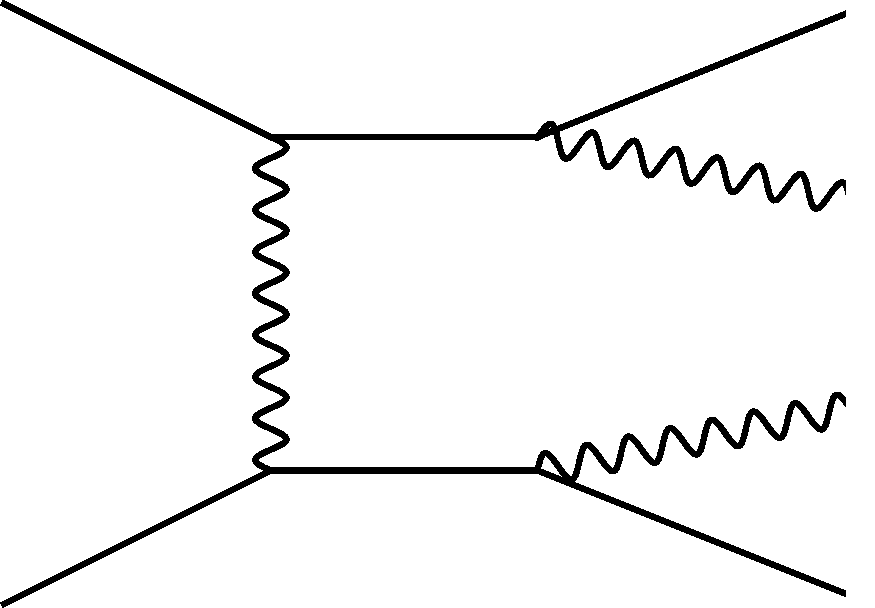
\includegraphics[width=0.3\textwidth]{figures/samples/feynEWKnonVBS6.pdf}}
\subfloat[]{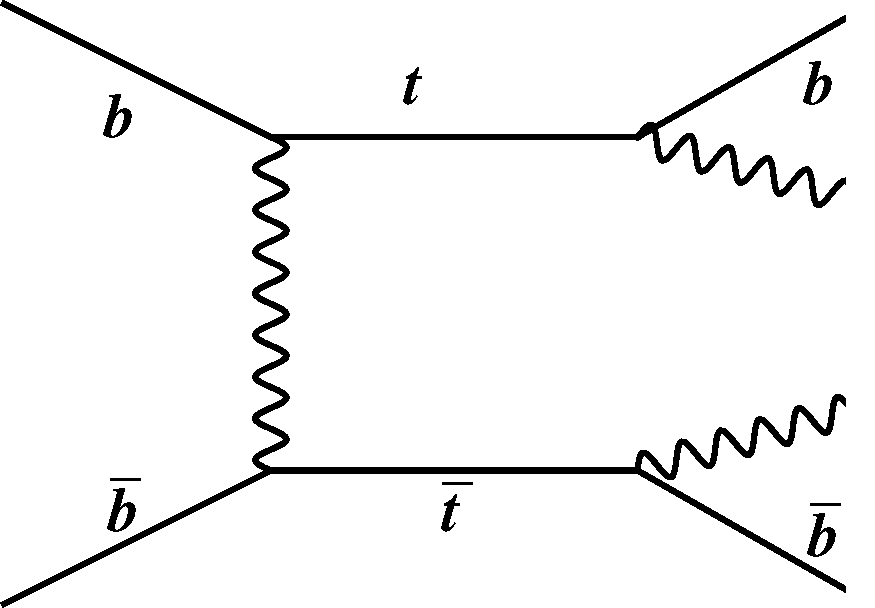
\includegraphics[width=0.3\textwidth]{figures/samples/feynEWKnonVBS1.pdf}}
\subfloat[]{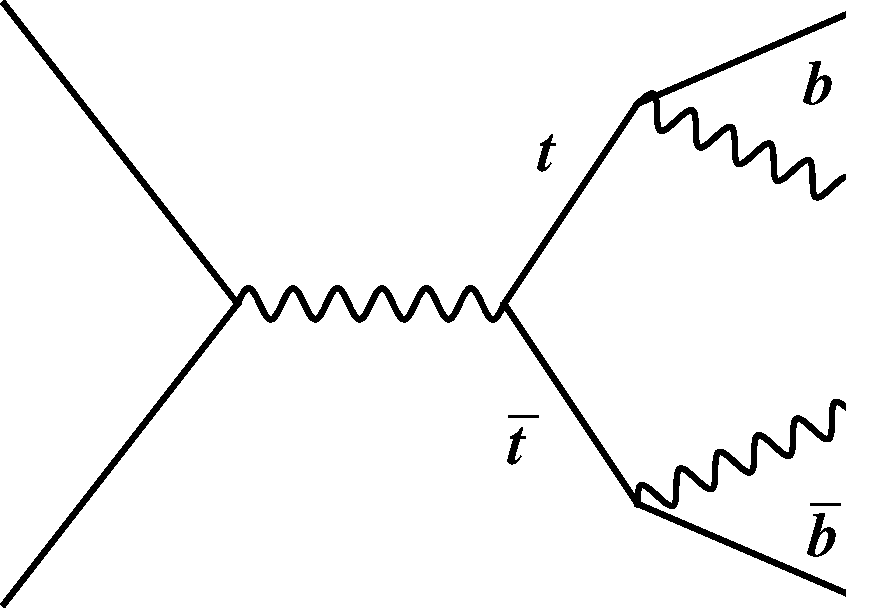
\includegraphics[width=0.3\textwidth]{figures/samples/feynEWKnonVBS2.pdf}}\\
\subfloat[]{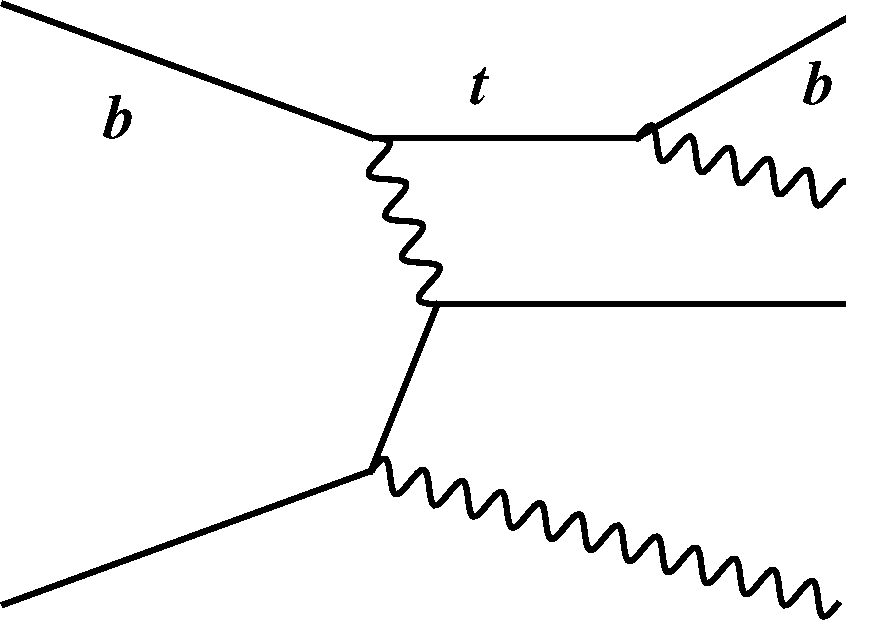
\includegraphics[width=0.3\textwidth]{figures/samples/feynEWKnonVBS7.pdf}}
\caption{
Examples of non-VBS $\mathcal{O}(\alpha_{EW}^6)$ diagrams contributin to the signal.
}
\label{fig:feynmanEWKnonVBS}
\end{center}
\end{figure}

%semileptonic and 1-lepton
Depending on the decay products of the vector bosons, VBS processes can be categorized into three types: fully leptonic, fully hadronic, and semileptonic. 
The fully leptonic VBS analysis studies final states where both vector bosons decay into leptons. 
Similarly, the fully hadronic analysis targets cases where the decay products are exclusively hadronic.
While studies of fully leptonic final states have been done, the branching ratio from double leptonic decay modes is relatively small. On the other hand, fully hadronic final states have a significantly higher branching ratio but introduce considerable background noise, making them challenging to analyze.
The semileptonic VBS analysis is looking at final states with one hadronic and one leptonic boson, offering a balanced compromise between a higher branching ratio and manageable background levels. As illustrated in Figure~\ref{fig:semi_vbs}, the two ``forward'' jets, $j_{f}$ and $j_{b}$, are high \pt jets that scatter through the coupling of the gauge bosons. These jets, pointing roughly along the beamline direction, serve as signatures of the VBS process. Further details on physics object definitions and VBS selection criteria will be discussed in Chapter~\ref{chap:objects_def} and Section~\ref{subsec:vbs_selection}.

Figure~\ref{fig:semi_vbs} also shows two jets, $j_{c}$, orginating from the hadronically decaying vector boson. 
The boson decaying leptonically can have a few conbinations of decay products. 
By counting the number of oberverable lepton(s), we have three channels in the semileptonic VBS analysis. 
Although neutrinos are technically leptons, within the context of this and similar analyses, ``lepton'' typically refers to those detectable directly by the ATLAS and CMS detectors.
Therefore, the 0-lepton channel corresponds to final states where the vector boson decays into a pair of neutrinos.
The 1-lepton channel involves one observable lepton (e.g., $e$, $\mu$) and a neutrino, while the 2-lepton channel includes final states without neutrinos. Most of the work presented in this thesis applies to all three channels but is primarily discussed from the 1-lepton channel perspective.

%Therefore, the 0-lepton channel is refering to the final states which the vector boson decay into a pair of neutrinos. The 1-lepton channel is one oberservable lepton (ie, $e$, $\mu$) and a neutrino, and the 2-lepton channel has no neutrinos. Most of the works mentioned in this thesis are generally applied to all 3 channels, but will be told from the 1-lepton channel's perspect.
%While neutrinos are leptons by definitions. In the context of this and similar analyses, lepton usually refers to the ones that can be detected directly by the ATLAS and CMS detectors. 

\begin{figure}[tbp]
\centering
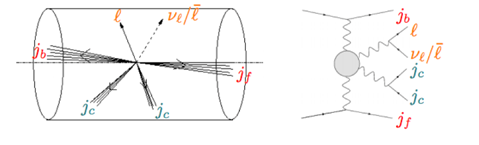
\includegraphics[width=0.75\textwidth]{figures/theory/semi_vbs.png}
\caption{
A schematic representation of a semileptonic VBS process within the detector, accompanied by the corresponding Feynman diagram.
}
\label{fig:semi_vbs}
\end{figure}

%Without the Higgs mechanism, calculations for VBS would lead to probabilities that exceed 100\% at high energies and violate unitarity. The discovery of a Higgs boson in LHC motivates further study of the mechanism of EWSB by probing the vector boson scattering (VBS) process. This process involves a quartic gauge coupling (QGC) vertex (Figure 2). The QGC is the self-coupling among four electroweak gauge bosons. The mechanism responsible for EWSB must also regularize the cross-section of SM VBS to restore unitarity above 1 TeV. Various physics models beyond the SM (BSM) predict enhancements of VBS production[6,7]. Therefore, the measurements of VBS at high energy are crucial tests of the SM and will determine whether the Higgs is entirely responsible for EWSB.

%%\begin{figure}[htbp]
%%\centering
%%\begin{subfigure}{.3\textwidth}
%%  \centering
%%\begin{tikzpicture}
%%  \begin{feynman}
%%    \vertex (a);
%%    \vertex [above left=of a] (i1) {\(V_L\)};
%%    \vertex [below left=of a] (i2) {\(V_L\)};
%%    \vertex [above right=of a] (f1) {\(V_L\)};
%%    \vertex [below right=of a] (f2) {\(V_L\)};
%%
%%    \diagram* {
%%      (i1) -- [boson] (a) -- [boson] (f1),
%%      (i2) -- [boson] (a) -- [boson] (f2),
%%    };
%%  \end{feynman}
%%\end{tikzpicture}
%%\end{subfigure}%
%%\begin{subfigure}{.3\textwidth}
%%  \centering
%%\begin{tikzpicture}
%%  \begin{feynman}
%%    \vertex (a);
%%    \vertex [above left=of a] (i1) {\(V_L\)};
%%    \vertex [below left=of a] (i2) {\(V_L\)};
%%    \vertex [right=of a] (b);
%%    \vertex [above right=of b] (f1) {\(V_L\)};
%%    \vertex [below right=of b] (f2) {\(V_L\)};
%%
%%    \diagram* {
%%      (i1) -- [boson] (a) -- [boson] (b)-- [boson] (f1),
%%      (i2) -- [boson] (a),
%%      (f2) -- [boson] (b),
%%    };
%%  \end{feynman}
%%\end{tikzpicture}
%%\end{subfigure}%
%%\begin{subfigure}{.3\textwidth}
%%  \centering
%%\begin{tikzpicture}
%%  \begin{feynman}
%%    \vertex (a);
%%    \vertex [above left=of a] (i1) {\(V_L\)};
%%    \vertex [above right=of a] (i2) {\(V_L\)};
%%    \vertex [below=of a] (b);
%%    \vertex [below left=of b] (f1) {\(V_L\)};
%%    \vertex [below right=of b] (f2) {\(V_L\)};
%%
%%    \diagram* {
%%      (i1) -- [boson] (a) -- [boson] (b)-- [boson] (f1),
%%      (i2) -- [boson] (a),
%%      (f2) -- [boson] (b),
%%    };
%%  \end{feynman}
%%\end{tikzpicture}
%%\end{subfigure}
%%
%%\vspace{2cm}
%%\begin{subfigure}{.3\textwidth}
%%  \centering
%%\begin{tikzpicture}
%%  \begin{feynman}
%%    \vertex (a);
%%    \vertex [above left=of a] (i1) {\(V_L\)};
%%    \vertex [below left=of a] (i2) {\(V_L\)};
%%    \vertex [right=of a] (b);
%%    \vertex [above right=of b] (f1) {\(V_L\)};
%%    \vertex [below right=of b] (f2) {\(V_L\)};
%%
%%    \diagram* {
%%      (i1) -- [boson] (a) -- [scalar, edge label=\(H\)] (b)-- [boson] (f1),
%%      (i2) -- [boson] (a),
%%      (f2) -- [boson] (b),
%%    };
%%  \end{feynman}
%%\end{tikzpicture}
%%\end{subfigure}
%%\begin{subfigure}{.3\textwidth}
%%  \centering
%%\begin{tikzpicture}
%%  \begin{feynman}
%%    \vertex (a);
%%    \vertex [above left=of a] (i1) {\(V_L\)};
%%    \vertex [above right=of a] (i2) {\(V_L\)};
%%    \vertex [below=of a] (b);
%%    \vertex [below left=of b] (f1) {\(V_L\)};
%%    \vertex [below right=of b] (f2) {\(V_L\)};
%%
%%    \diagram* {
%%      (i1) -- [boson] (a) -- [scalar, edge label=\(H\)] (b)-- [boson] (f1),
%%      (i2) -- [boson] (a),
%%      (f2) -- [boson] (b),
%%    };
%%  \end{feynman}
%%\end{tikzpicture}
%%\end{subfigure}
%%\caption{The tree-level Feynman diagrams contributing to VBS process.}
%%\label{fig:feynman_diagrams}
%%\end{figure}




\clearpage
\section{Beyond the Standard Model}
%aQGCs
Despite intensive searches, experiments at the LHC have not yet observed new physics phenomena beyond those predicted by the Standard Model of particle physics.
After the discovery of the Higgs boson, a significant number of analyses have been dedicated to searching for traces of new particles. In the meantime, we also explore the possibility of Beyond the Standard Model (BSM) interactions involving known Standard Model particles, such as the Higgs, $W$, and $Z$ bosons. Any potential new physics related to EWSB could thus modify the interactions of these particles.
In our case where no new physics has yet been found, the Standard Model can be considered as a low-energy approximation of a more comprehensive theory.
This perspective allows us to describe potential BSM phenomena through an Effective Field Theory (EFT)  approach~\cite{Weinberg:1978kz}~\cite{RevModPhys.52.515}.

\subsection{Anomalous Quartic Gauge Couplings}
\label{Anomalous_Quartic_Gauge_Couplings}

The concept of anomalous couplings among electroweak vector bosons existed before the Higgs boson was discovered~\cite{GaemersGounaris1979}. Even then, it was widely believed that EWSB governed the electroweak interactions, ensuring they remained consistent without violating any unitarity constraints.
Given the discovery of the Higgs boson and the solid foundation of the $\mathrm{SU}(3)_C \otimes \mathrm{SU}(2)_L \otimes \mathrm{U}(1)_Y$ gauge symmetry, employing an EFT approach has emerged as a compelling method for predicting and analyzing precise measurements of electroweak processes, including any deviations from expected results.

The EFT framework offers a streamlined and versatile way to explore anomalous couplings without being tied to any specific model~\cite{Degrande_2013}. This includes both anomalous triple gauge couplings (aTGCs) and anomalous quartic gauge couplings (aQGCs). Although aTGCs remain a significant area of interest, our focus here will be aQGCs. aQGCs are particularly intriguing because they can be investigated through VBS, providing a clear pathway for probing these potential deviations.

Assuming that new physics emerges only at energies above the scale $\Lambda$, we can describe any phenomena beyond the Standard Model (including anomalous gauge couplings) using an effective Lagrangian:
\begin{equation}
\mathcal{L}_{\text{eff}} = \mathcal{L}_{\text{SM}} + \sum_i \frac{c^{(6)}_i}{\Lambda^2} \mathcal{O}^{(6)}_i + \sum_j \frac{c^{(8)}_j}{\Lambda^4} \mathcal{O}^{(8)}_j + \ldots
\end{equation} 
where $\mathcal{L}_{\text{SM}}$ is the Standard Model Lagrangian, $\mathcal{O}_i$ are the higher-dimensional operators of dimension $d_i$, $c_i$ are the Wilson coefficients.
In the effective Lagrangian, we include only even-dimensional operators because odd-dimensional operators would violate lepton and/or baryon number conservation~\cite{Degrande_2013}. 
The dimension-6 (D-6) terms, $\frac{c^{(6)}_i}{\Lambda^2} \mathcal{O}^{(6)}_i$, are often associated with aTGCs. 
The dimension-8 (D-8) terms, $\frac{c^{(8)}_j}{\Lambda^4} \mathcal{O}^{(8)}_j$, are typically associated with aQGCs, introducing or modifying interactions involving four gauge bosons.
Although both D-6 and D-8 operators can contribute to the VBS processes, the D-6 operators have been tightly constrained to values around zero by previous diboson measurements. Therefore, we will focus our discussion on the D-8 operators here.


Building on the EFT approach to model the effects of possible aQGCs, we adopt the Eboli model, which introduces 21 new D-8 operators adhering to the SM $SU(2)\times U(1)_Y$ gauge symmetry~\cite{eboli2006p}.
These operators can be classified into three categories: scalar, tensor, and mixed types. A list of these operators is provided at the end of this section.
As shown in Table~\ref{table:eboli_op}, the semileptonic VBS stands out as an exceptional process capable of testing nineteen D-8 operators concurrently, with final states that involved $WW$, $WZ$, and $ZZ$ boson pairs.

\begin{table}[h!]
	\centering
	\begin{tabular}{|c|c|c|c||c|c|c|c|c|c|}
		\hline
		& WWWW & WWZZ & ZZZZ & WW$\gamma$Z & WW$\gamma\gamma$ & ZZZ$\gamma$ & ZZ$\gamma\gamma$ & Z$\gamma\gamma\gamma$ & $\gamma\gamma\gamma\gamma$ \\ \hline
		$\mathcal{L}_{S0,2}, \mathcal{L}_{S1}$ & X & X & X & — & — & — & — & — & — \\ \hline
		$\mathcal{L}_{M0}, \mathcal{L}_{M1}, \mathcal{L}_{M6}, \mathcal{L}_{M7}$ & X & X & X & X & X & X & X & — & — \\ \hline
		$\mathcal{L}_{M2}, \mathcal{L}_{M3}, \mathcal{L}_{M4}, \mathcal{L}_{M5}$ & — & X & X & X & X & X & X & — & — \\ \hline
		$\mathcal{L}_{T0}, \mathcal{L}_{T1}, \mathcal{L}_{T2}$ & X & X & X & X & X & X & X & X & X \\ \hline
		$\mathcal{L}_{T5}, \mathcal{L}_{T6}, \mathcal{L}_{T7}$ & — & X & X & X & X & X & X & X & X \\ \hline
		$\mathcal{L}_{T8}, \mathcal{L}_{T9}$ & — & — & X & — & — & — & X & X & X \\ \hline
	\end{tabular}
	\caption{Correspondences between the vertices and operators. The ``X'' marks indicate the quartic gauge vertices that can be modified by the specified D-8 operators.}
	\label{table:eboli_op}
\end{table}


%%%%%%%%%%%%%%%%%%%%%%%%%%%%%%%%%
The following are the three classes of D-8 operators in the Eboli model~\cite{eboli2006p}.

The scalar operators containing just covariant derivatives of the Higgs field, $D_\mu\Phi$:
\begin{eqnarray}
  {\cal L}_{S0,2} &=& \left [ \left ( D_\mu \Phi \right)^\dagger
 D_\nu \Phi \right ] \times
\left [ \left ( D^\mu \Phi \right)^\dagger
D^\nu \Phi \right ]
\\
  {\cal L}_{S1} &=& \left [ \left ( D_\mu \Phi \right)^\dagger
 D^\mu \Phi  \right ] \times
\left [ \left ( D_\nu \Phi \right)^\dagger
D^\nu \Phi \right ]
\end{eqnarray}
Here, the operators $\mathcal{L}_{S0}$ and $\mathcal{L}_{S2}$ are Hermitian conjugates, and can be treated as the same operator in practice.

The tensor operators containing just the field strength tensor:
\begin{eqnarray}
 {\cal L}_{T,0} &=&   \hbox{Tr}\left [ \hat{W}_{\mu\nu} \hat{W}^{\mu\nu} \right ]
\times   \hbox{Tr}\left [ \hat{W}_{\alpha\beta} \hat{W}^{\alpha\beta} \right ]
\\
 {\cal L}_{T,1} &=&   \hbox{Tr}\left [ \hat{W}_{\alpha\nu} \hat{W}^{\mu\beta} \right ]
\times   \hbox{Tr}\left [ \hat{W}_{\mu\beta} \hat{W}^{\alpha\nu} \right ]
\\
 {\cal L}_{T,2} &=&   \hbox{Tr}\left [ \hat{W}_{\alpha\mu} \hat{W}^{\mu\beta} \right ]
\times   \hbox{Tr}\left [ \hat{W}_{\beta\nu} \hat{W}^{\nu\alpha} \right ]
\\
 {\cal L}_{T,3} &=&   \hbox{Tr}\left [ \hat{W}_{\alpha\mu}
   \hat{W}^{\mu\beta}  \hat{W}^{\nu\alpha} \right ]
\times   B_{\beta\nu}
\\
 {\cal L}_{T,4} &=&   \hbox{Tr}\left [ \hat{W}_{\alpha\mu}
   \hat{W}^{\alpha\mu}  \hat{W}^{\beta\nu} \right ]
\times   B_{\beta\nu}
\\
 {\cal L}_{T,5} &=&   \hbox{Tr}\left [ \hat{W}_{\mu\nu} \hat{W}^{\mu\nu} \right ]
\times   B_{\alpha\beta} B^{\alpha\beta}
\\
 {\cal L}_{T,6} &=&   \hbox{Tr}\left [ \hat{W}_{\alpha\nu} \hat{W}^{\mu\beta} \right ]
\times   B_{\mu\beta} B^{\alpha\nu} 
\\
 {\cal L}_{T,7} &=&   \hbox{Tr}\left [ \hat{W}_{\alpha\mu} \hat{W}^{\mu\beta} \right ]
\times   B_{\beta\nu} B^{\nu\alpha} 
\\
 {\cal L}_{T,8} &=&   B_{\mu\nu} B^{\mu\nu}  B_{\alpha\beta} B^{\alpha\beta}
\\
 {\cal L}_{T,9} &=&  B_{\alpha\mu} B^{\mu\beta}   B_{\beta\nu} B^{\nu\alpha} 
\end{eqnarray}

The mixed operators containing $D_\mu\Phi$ and field strength:
\begin{eqnarray}
 {\cal L}_{M,0} &=&   \hbox{Tr}\left [ \hat{W}_{\mu\nu} \hat{W}^{\mu\nu} \right ]
\times  \left [ \left ( D_\beta \Phi \right)^\dagger
D^\beta \Phi \right ]
\\
 {\cal L}_{M,1} &=&   \hbox{Tr}\left [ \hat{W}_{\mu\nu} \hat{W}^{\nu\beta} \right ]
\times  \left [ \left ( D_\beta \Phi \right)^\dagger
D^\mu \Phi \right ]
\\
 {\cal L}_{M,2} &=&   \left [ B_{\mu\nu} B^{\mu\nu} \right ]
\times  \left [ \left ( D_\beta \Phi \right)^\dagger
D^\beta \Phi \right ]
\\
 {\cal L}_{M,3} &=&   \left [ B_{\mu\nu} B^{\nu\beta} \right ]
\times  \left [ \left ( D_\beta \Phi \right)^\dagger
D^\mu \Phi \right ]
\\
  {\cal L}_{M,4} &=& \left [ \left ( D_\mu \Phi \right)^\dagger \hat{W}_{\beta\nu}
 D^\mu \Phi  \right ] \times B^{\beta\nu}
\\
  {\cal L}_{M,5} &=& \left [ \left ( D_\mu \Phi \right)^\dagger \hat{W}_{\beta\nu}
 D^\nu \Phi  \right ] \times B^{\beta\mu}
\\
  {\cal L}_{M,6} &=& \left [ \left ( D_\mu \Phi \right)^\dagger \hat{W}_{\beta\nu}
\hat{W}^{\beta\nu} D^\mu \Phi  \right ] 
\\
  {\cal L}_{M,7} &=& \left [ \left ( D_\mu \Phi \right)^\dagger \hat{W}_{\beta\nu}
\hat{W}^{\beta\mu} D^\nu \Phi  \right ] 
\end{eqnarray}



